\section{Cherry picking}
\begin{frame}
    \frametitle{When to use cherry-pick}
    \begin{itemize}
        \item commit on the wrong branch
        \begin{itemize}
            \item cherry-pick it into the desired branch
            \item reset the orignal branch
        \end{itemize}
        \item you don't want to merge a whole branch
        \item as part of \texttt{git rebase}
    \end{itemize}
\end{frame}

\begin{frame}
    \frametitle{What does cherry-pick do}
    \begin{itemize}
        \item copies the content of the commit
        \item metadata like author and date are kept
    \end{itemize}
    \begin{alertblock}{Be aware of}
        \begin{itemize}
            \item changes the commit sha1
            \item different parents
        \end{itemize}
    \end{alertblock}
\end{frame}

\begin{frame}[fragile]
    \frametitle{What does rebase do}
    \begin{figure}
        \begin{center}
            \ifnumequal{\aspectratio}{43}
            {
                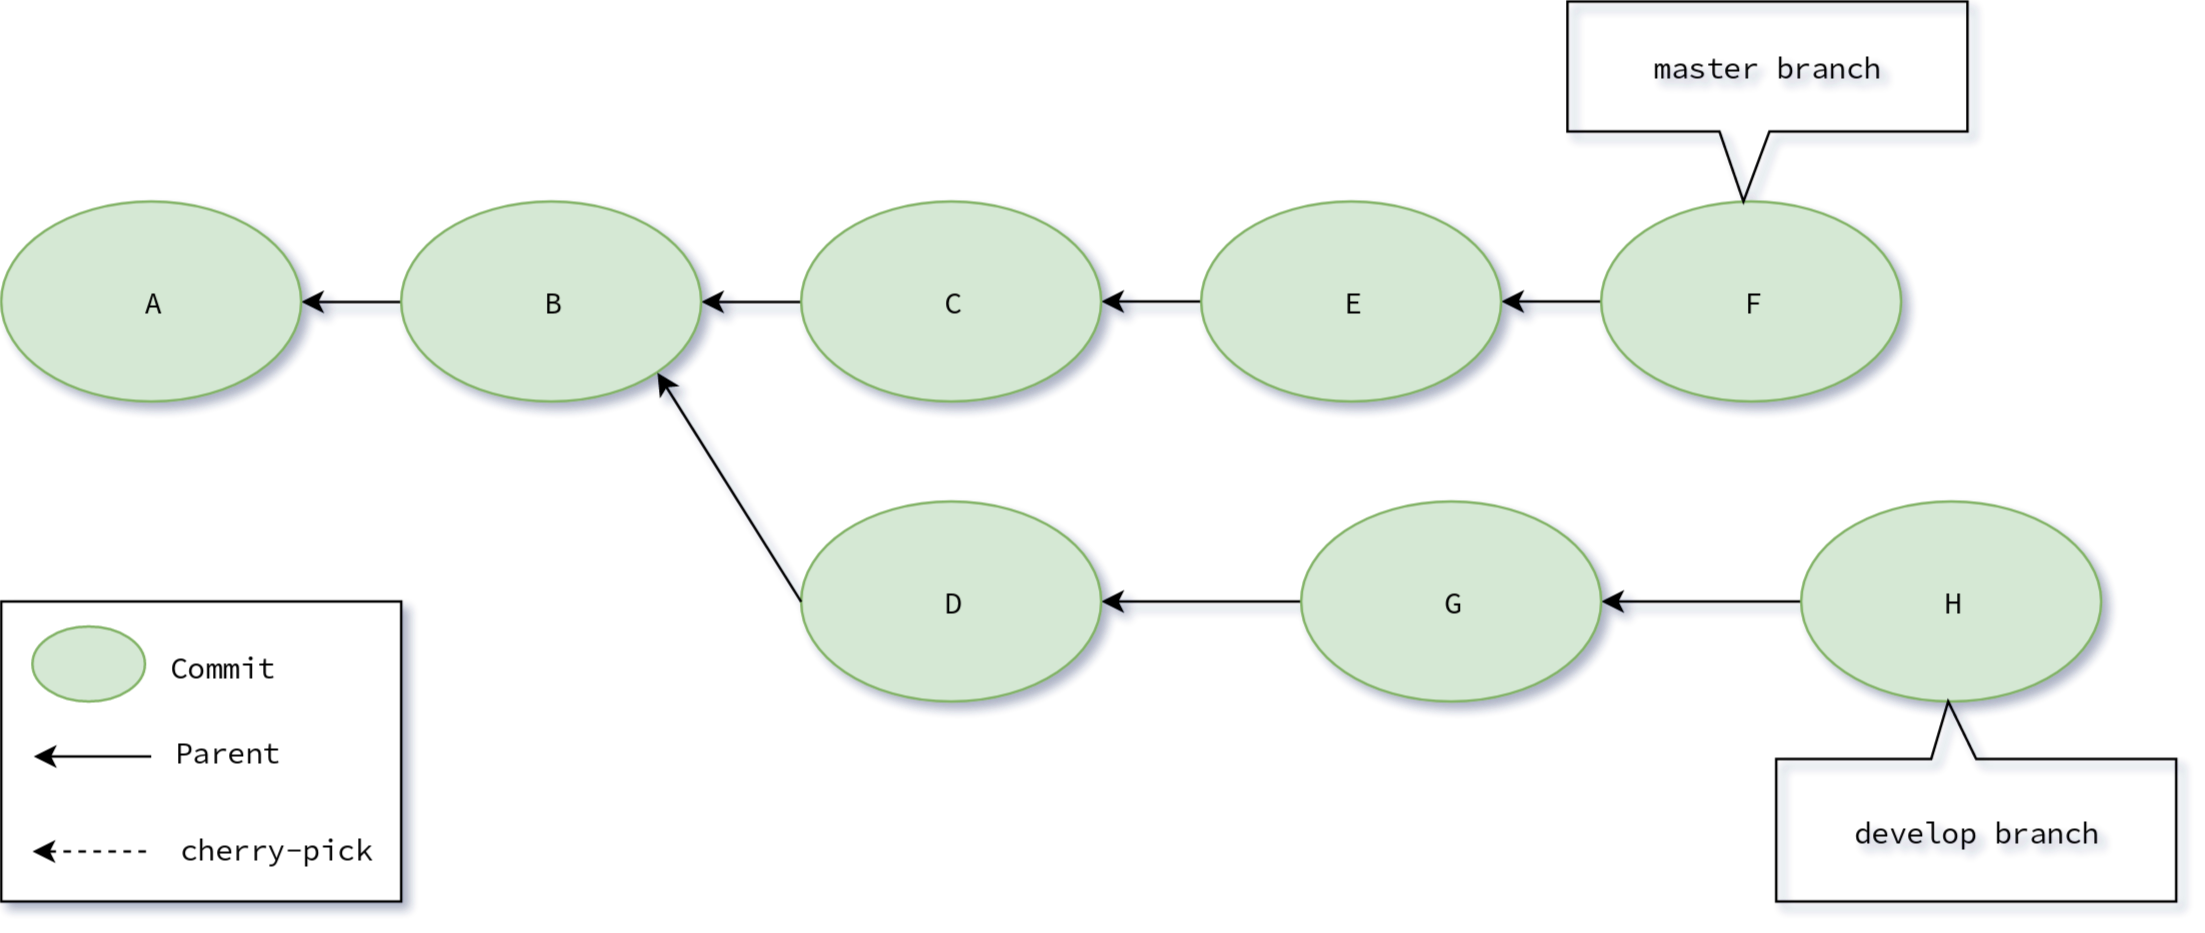
\includegraphics[width=1\textwidth,keepaspectratio]{./images/Rebase.png}
            }
            {
                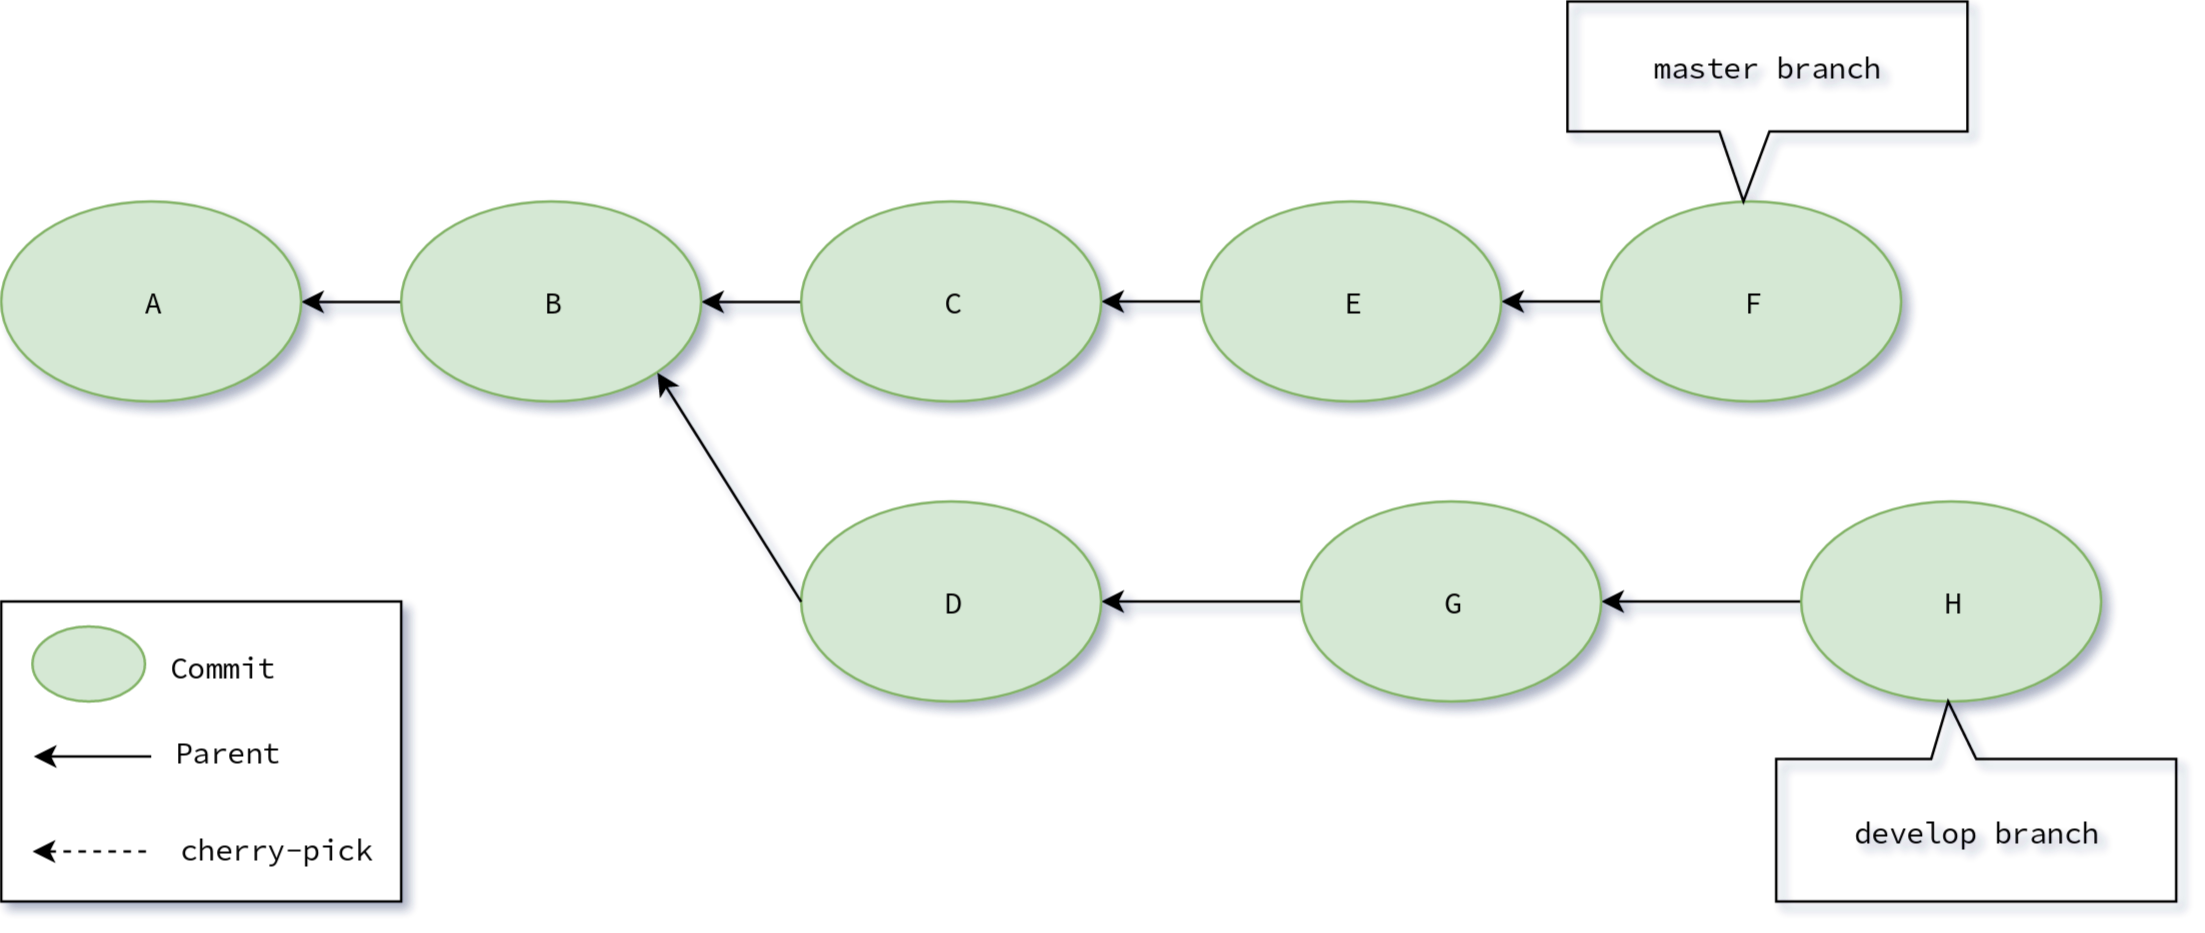
\includegraphics[height=0.75\textheight,keepaspectratio]{./images/Rebase.png}
            }
            \caption{Areas in git}
        \end{center}
    \end{figure}
\end{frame}

\begin{frame}[fragile]
    \frametitle{What does rebase do}
    \begin{figure}
        \begin{center}
            \ifnumequal{\aspectratio}{43}
            {
                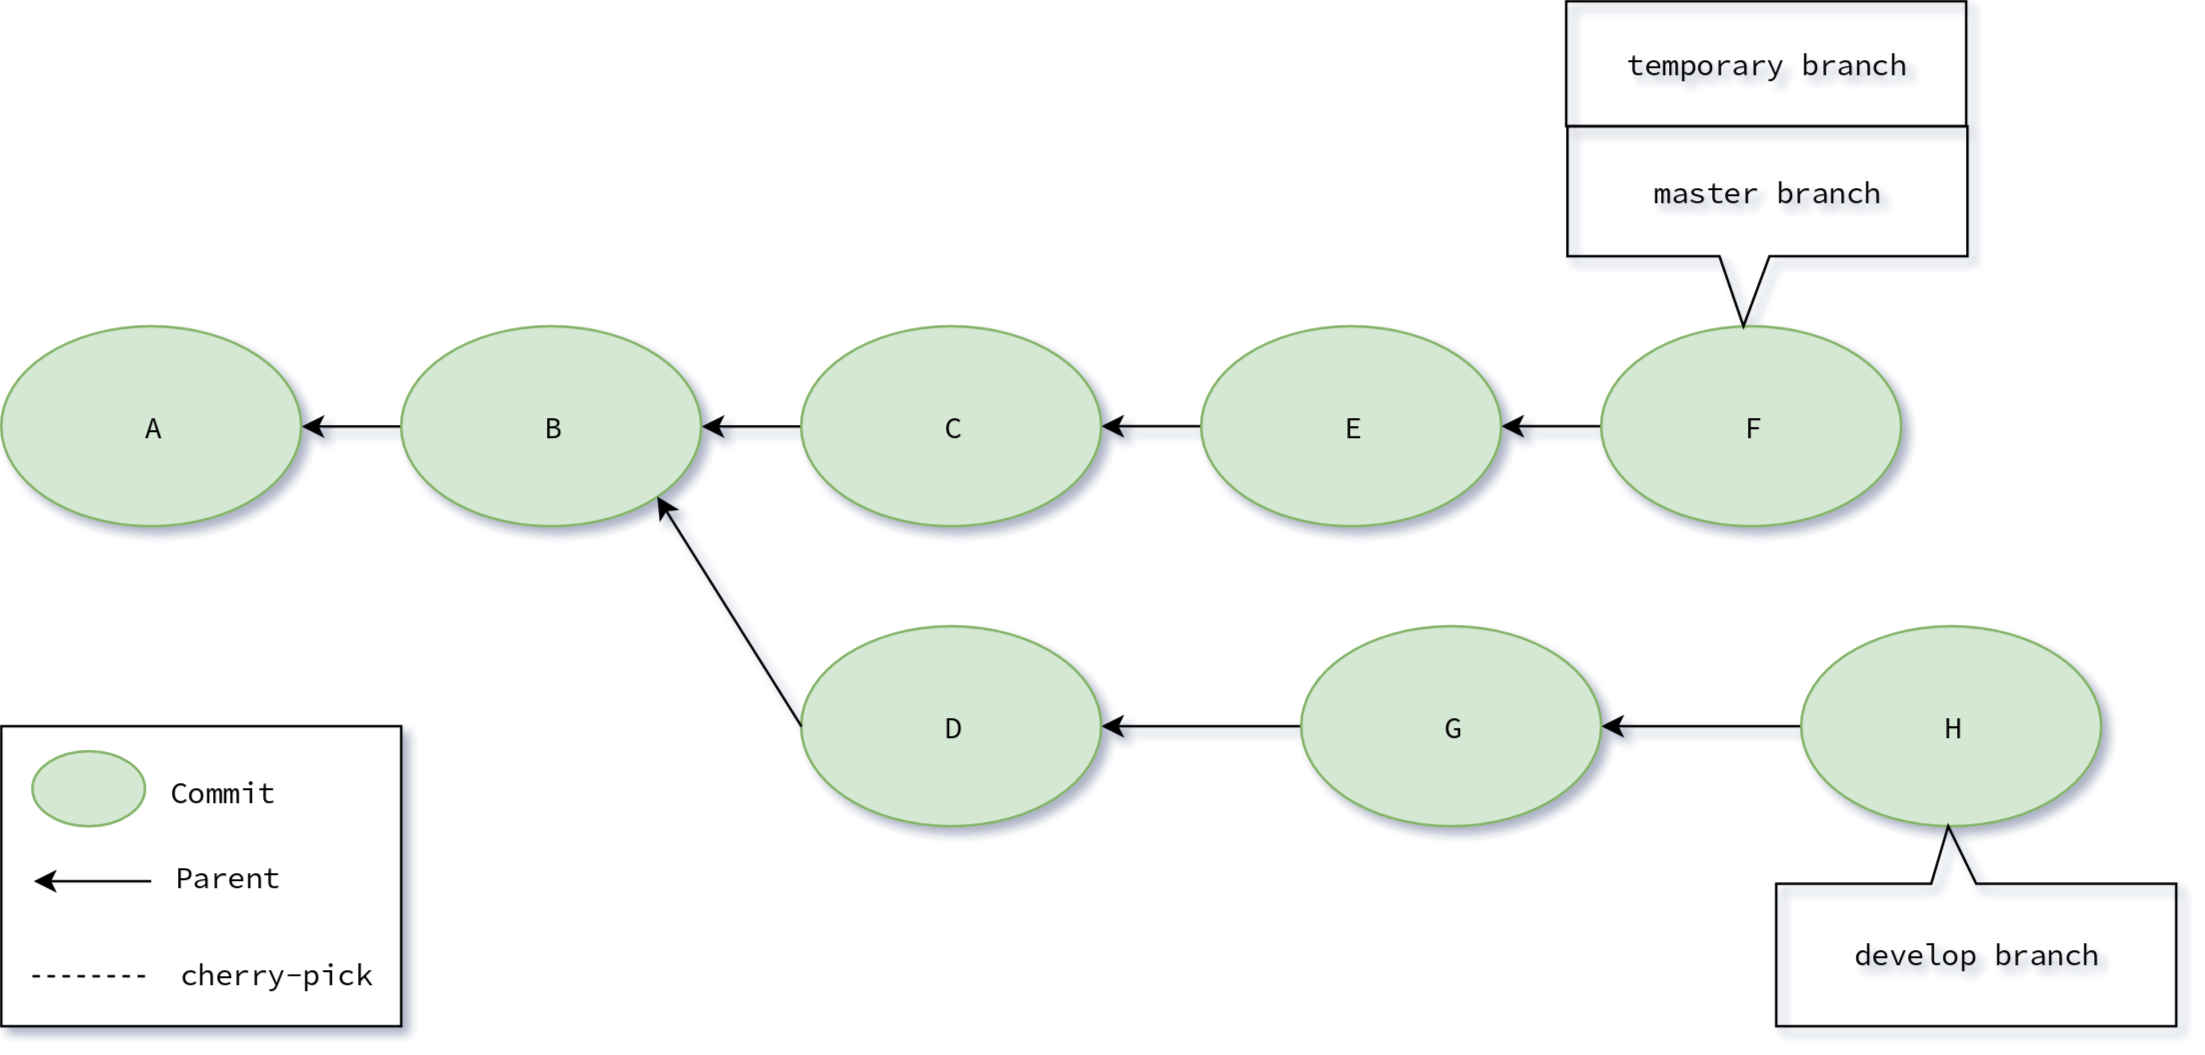
\includegraphics[width=1\textwidth,keepaspectratio]{./images/Rebase_TempBranch.png}
            }
            {
                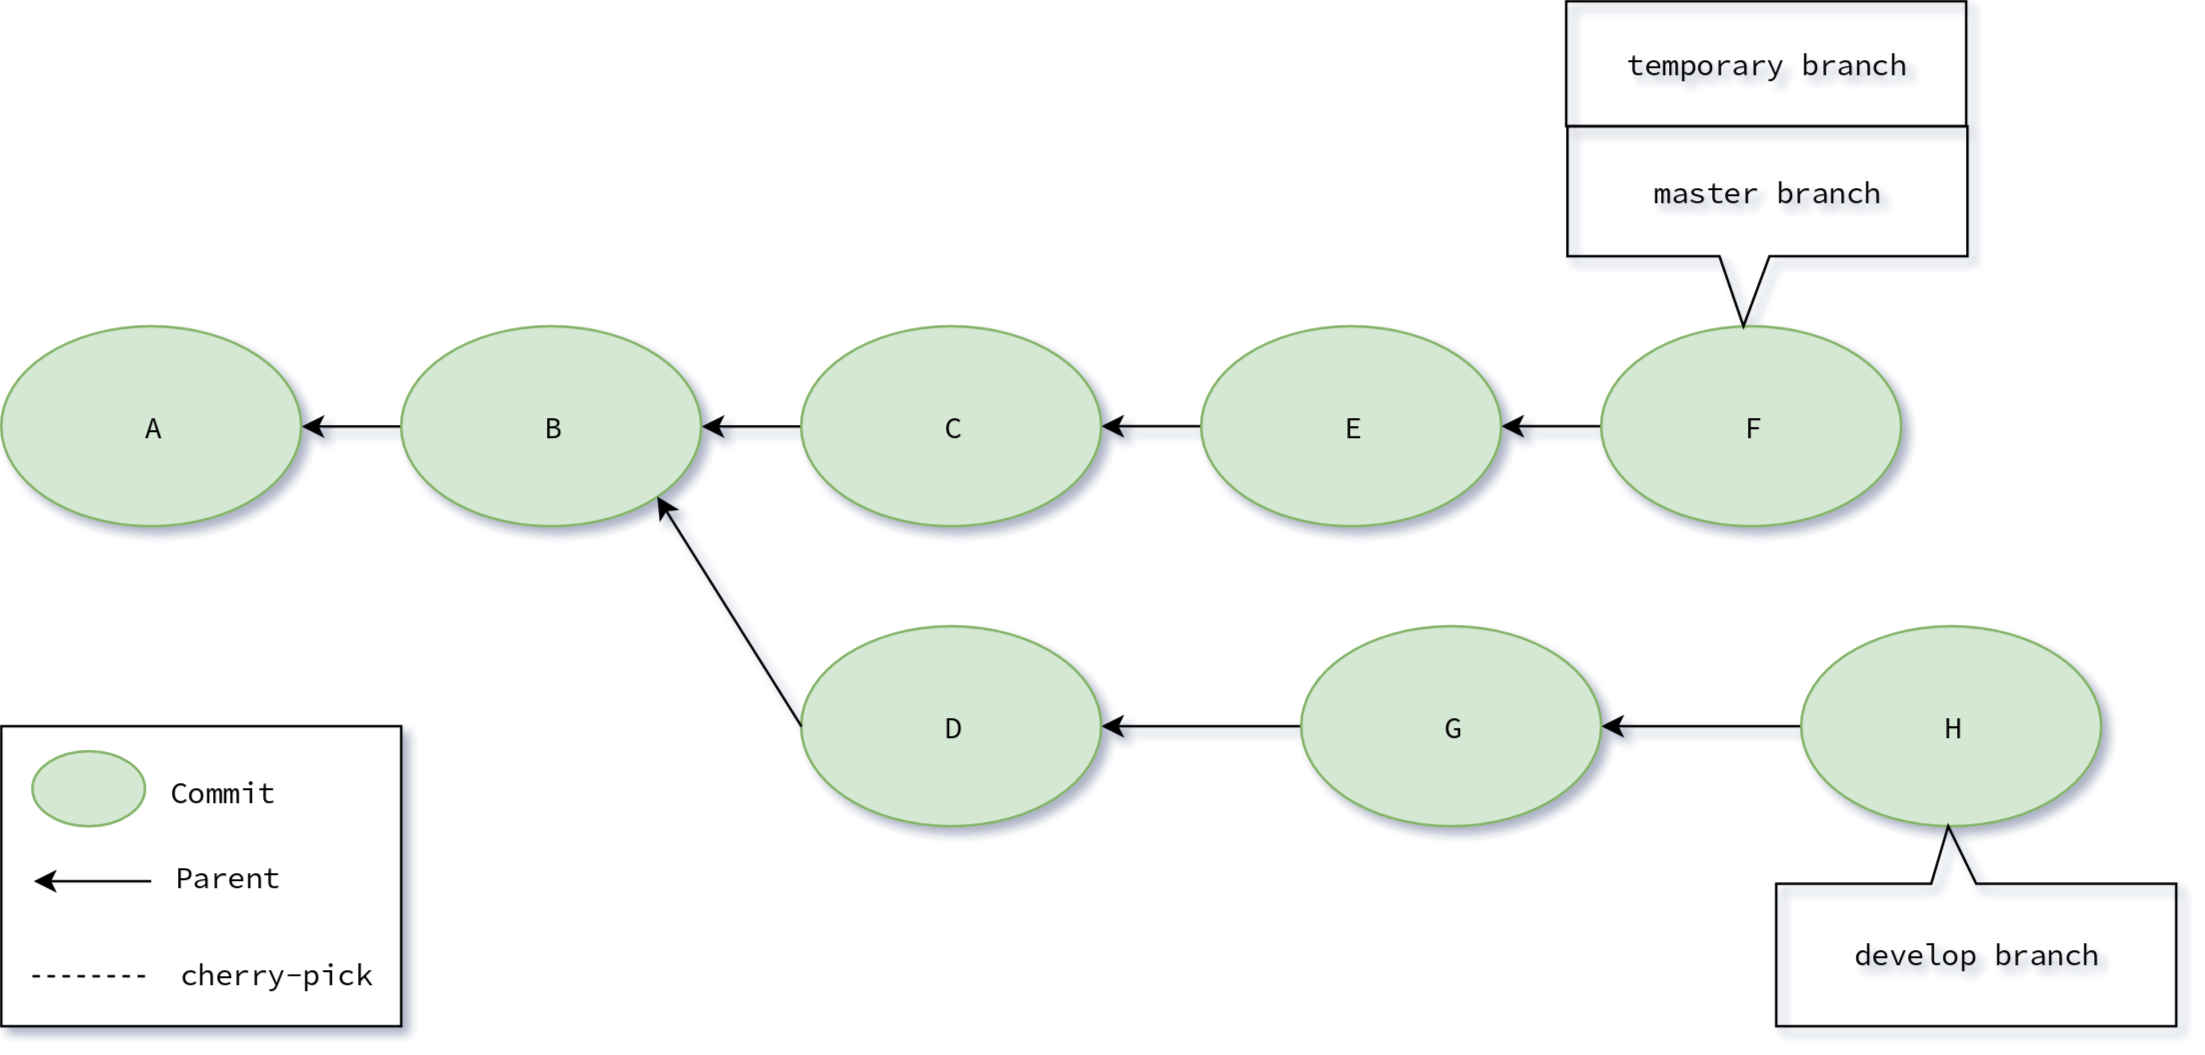
\includegraphics[height=0.75\textheight,keepaspectratio]{./images/Rebase_TempBranch.png}
            }
            \caption{Areas in git}
        \end{center}
    \end{figure}
\end{frame}

\begin{frame}[fragile]
    \frametitle{What does rebase do}
    \begin{figure}
        \begin{center}
            \ifnumequal{\aspectratio}{43}
            {
                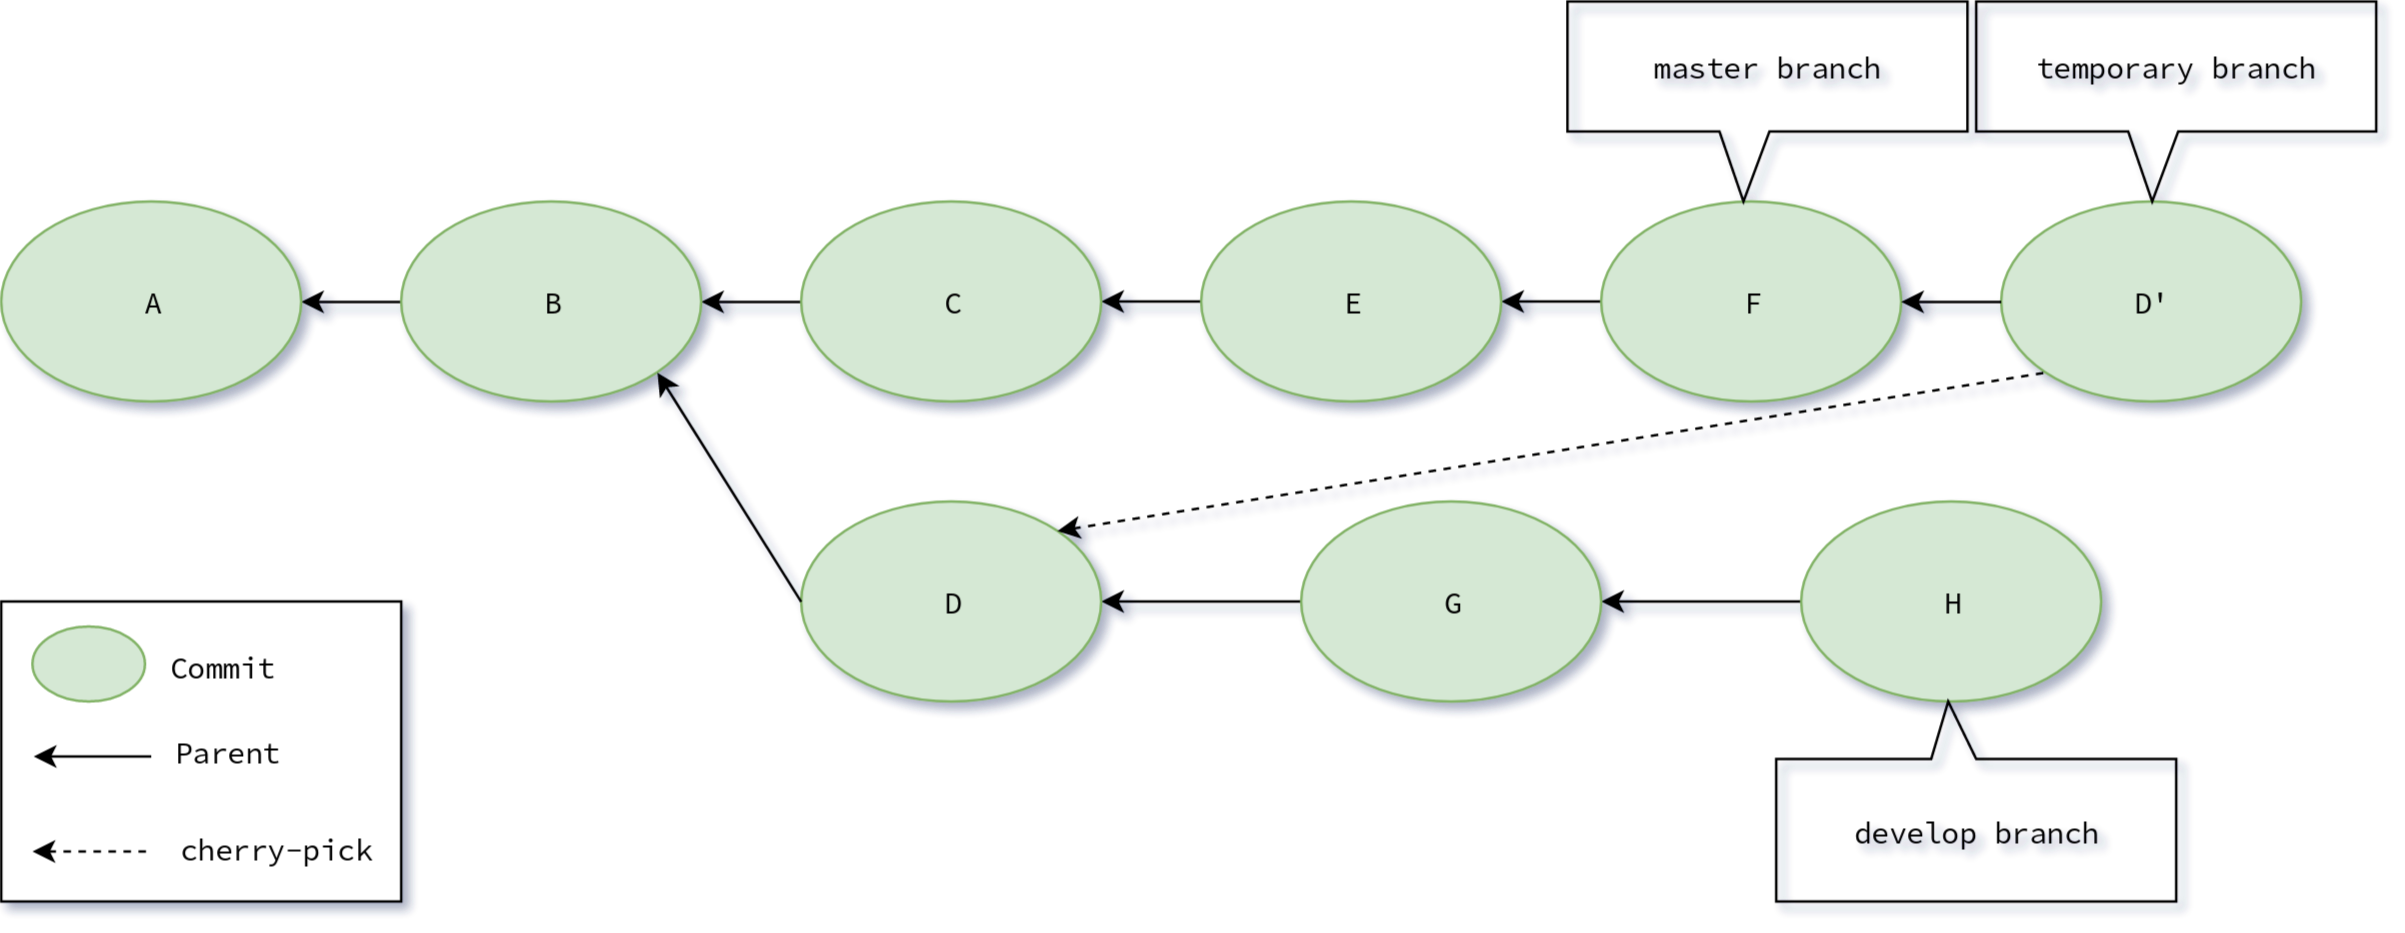
\includegraphics[width=1\textwidth,keepaspectratio]{./images/Rebase_FirstCherryPick.png}
            }
            {
                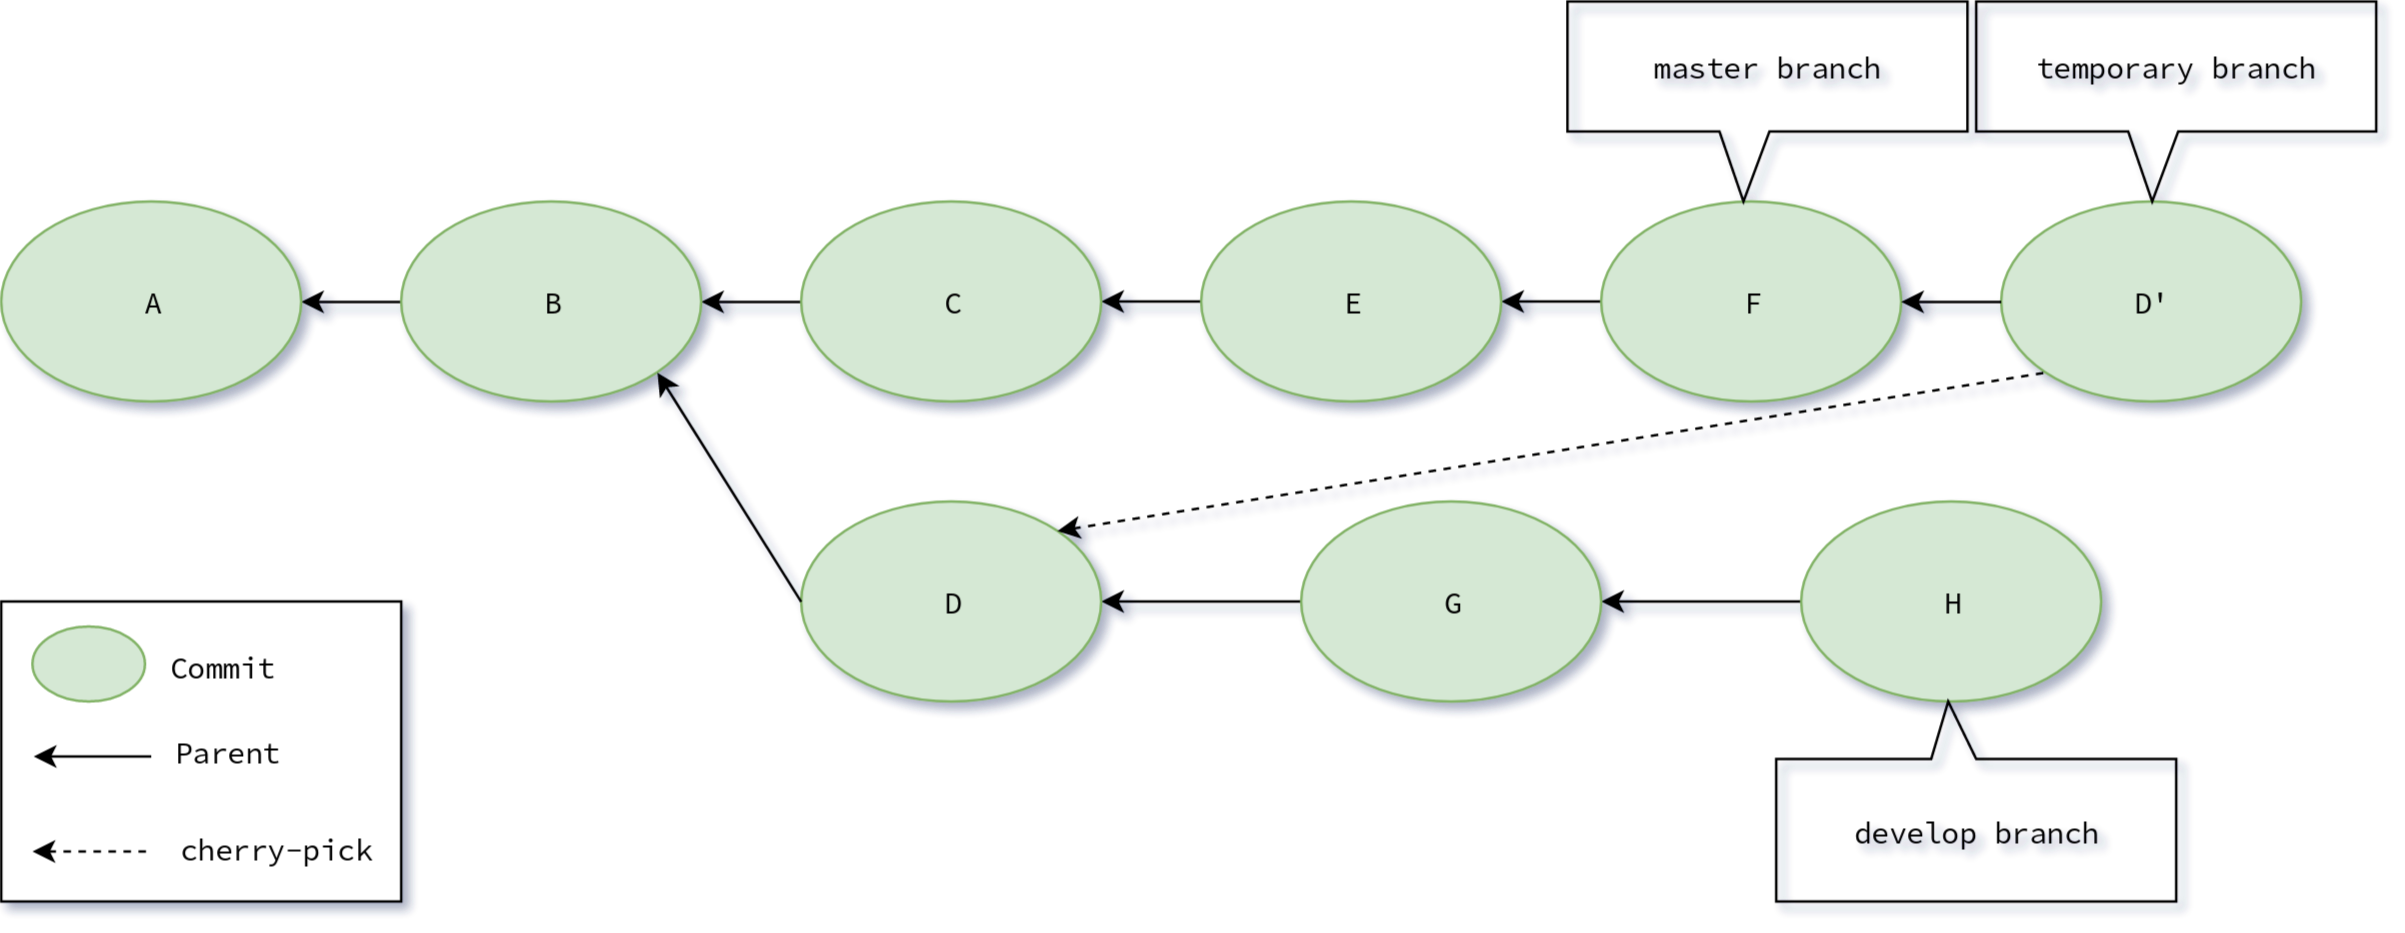
\includegraphics[width=0.9\textwidth,keepaspectratio]{./images/Rebase_FirstCherryPick.png}
            }
            \caption{Areas in git}
        \end{center}
    \end{figure}
\end{frame}

\begin{frame}[fragile]
    \frametitle{What does rebase do}
    \begin{figure}
        \begin{center}
            \ifnumequal{\aspectratio}{43}
            {
                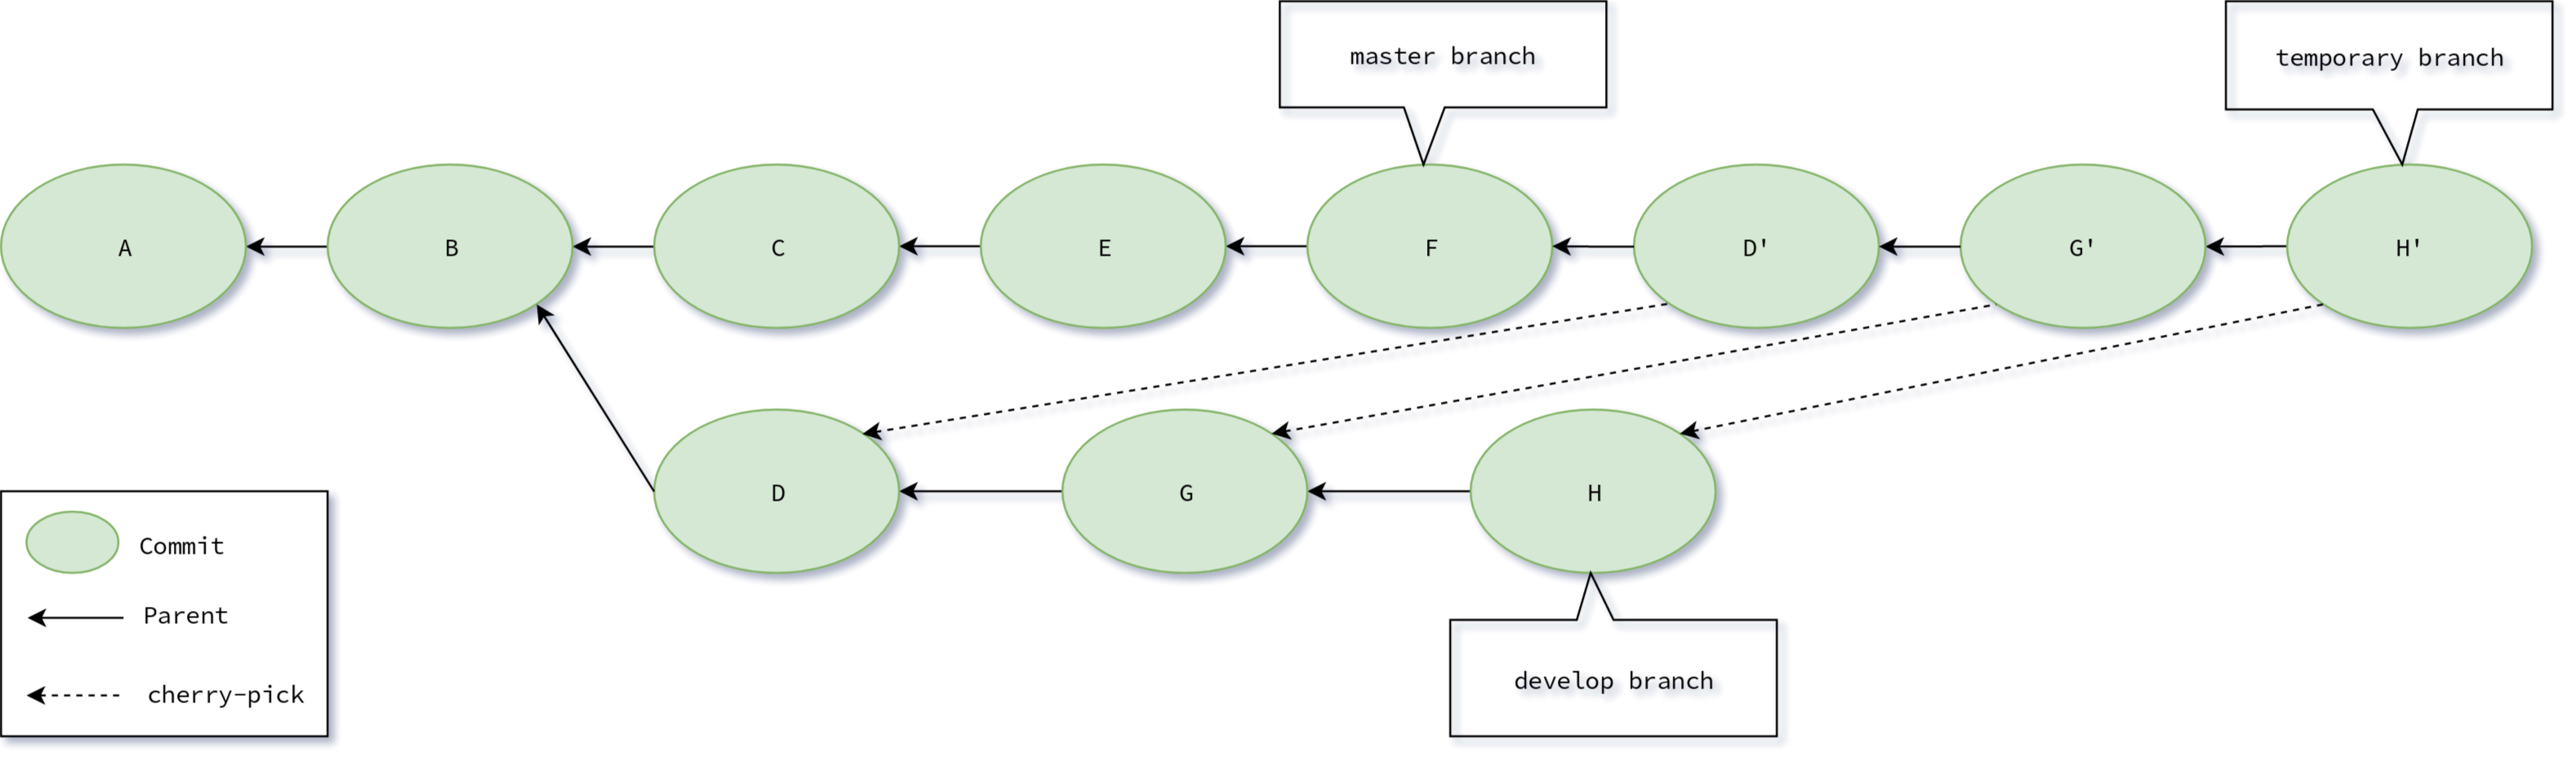
\includegraphics[width=1\textwidth,keepaspectratio]{./images/Rebase-Process.png}
            }
            {
                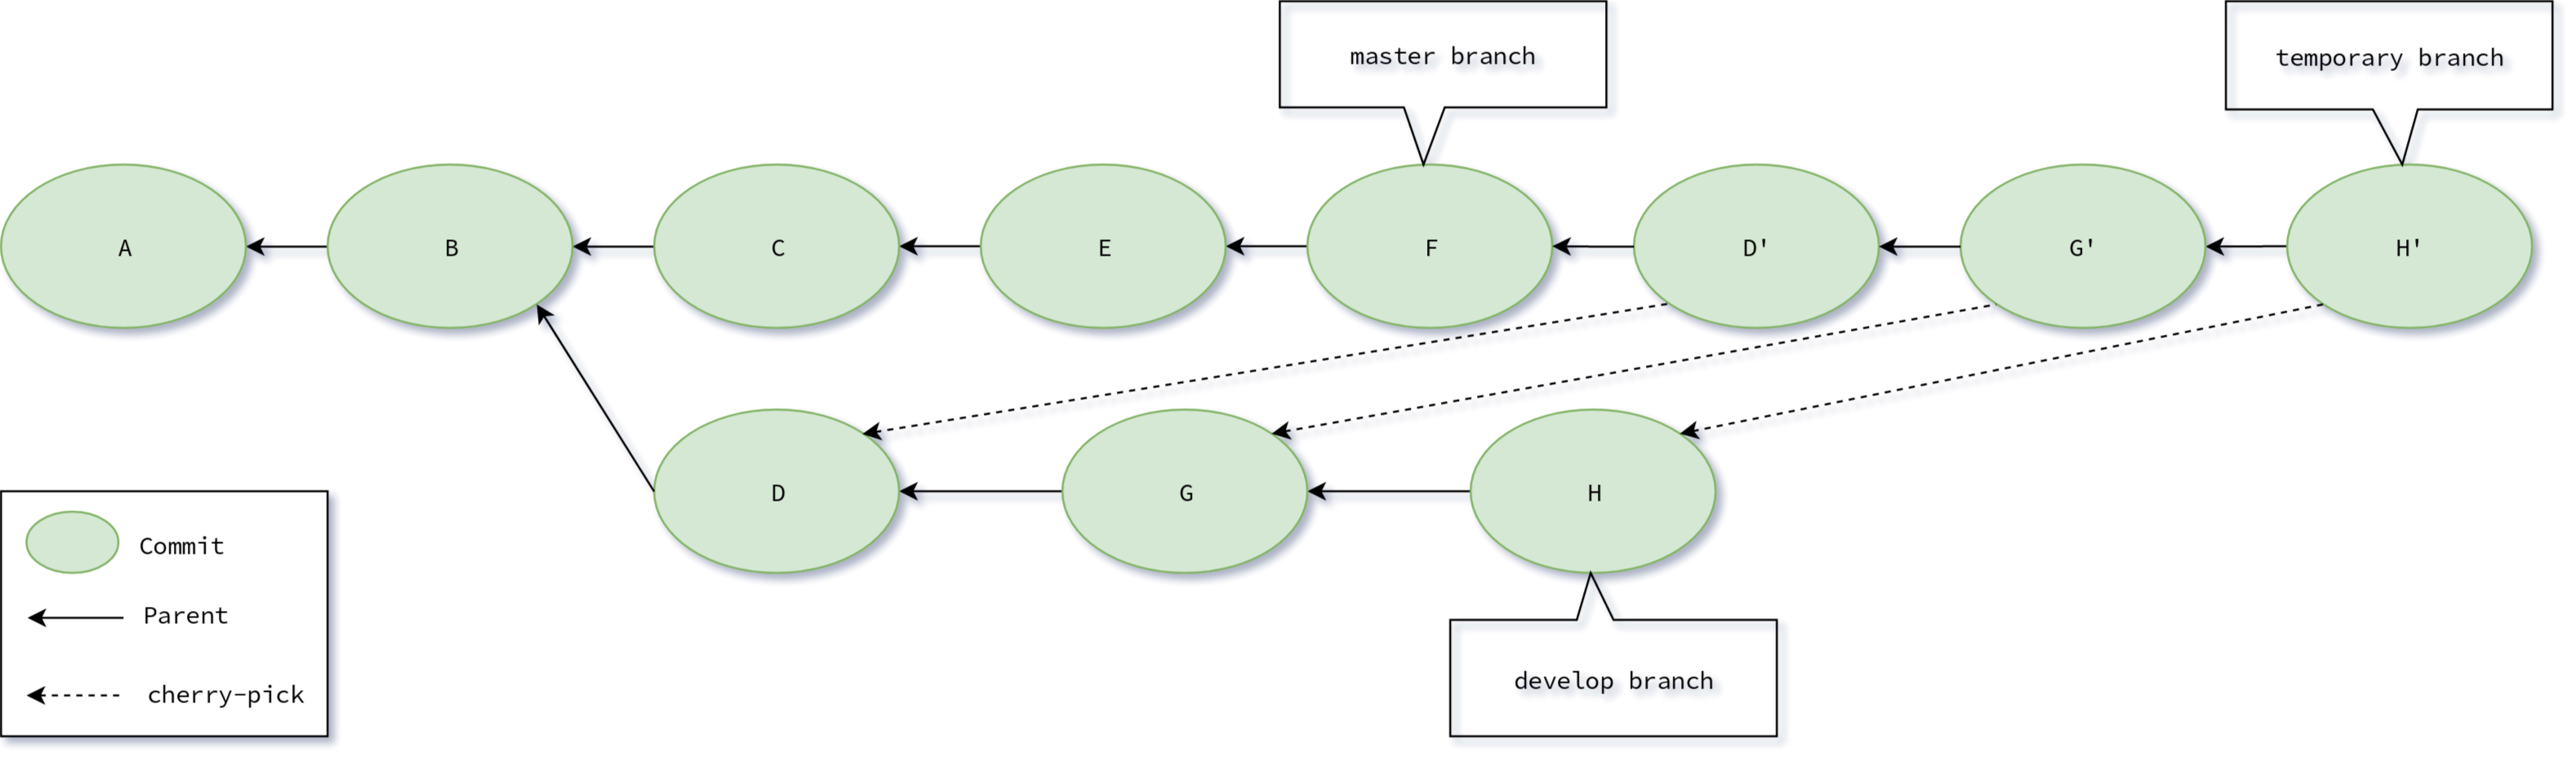
\includegraphics[width=1\textwidth,keepaspectratio]{./images/Rebase-Process.png}
            }
            \caption{Areas in git}
        \end{center}
    \end{figure}
\end{frame}

\begin{frame}[fragile]
    \frametitle{What does rebase do}
    \begin{figure}
        \begin{center}
            \ifnumequal{\aspectratio}{43}
            {
                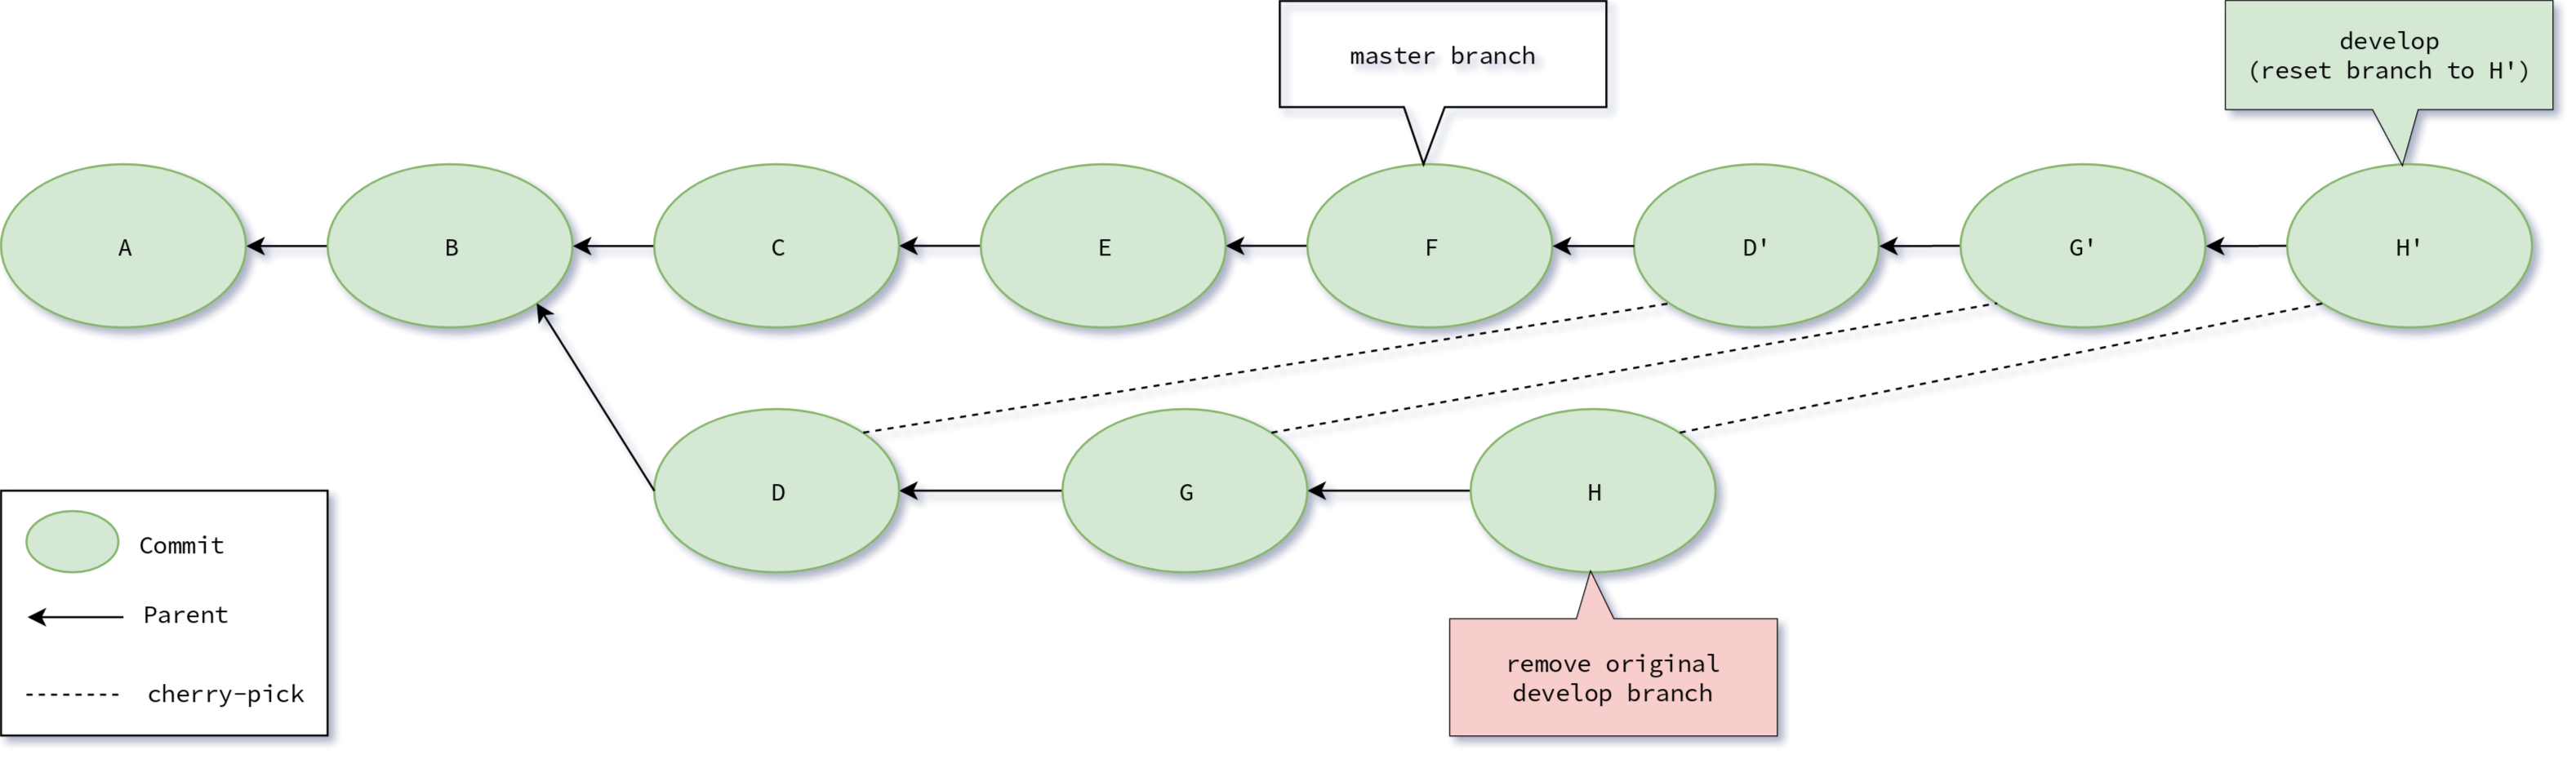
\includegraphics[width=1\textwidth,keepaspectratio]{./images/Rebase-Completed.png}
            }
            {
                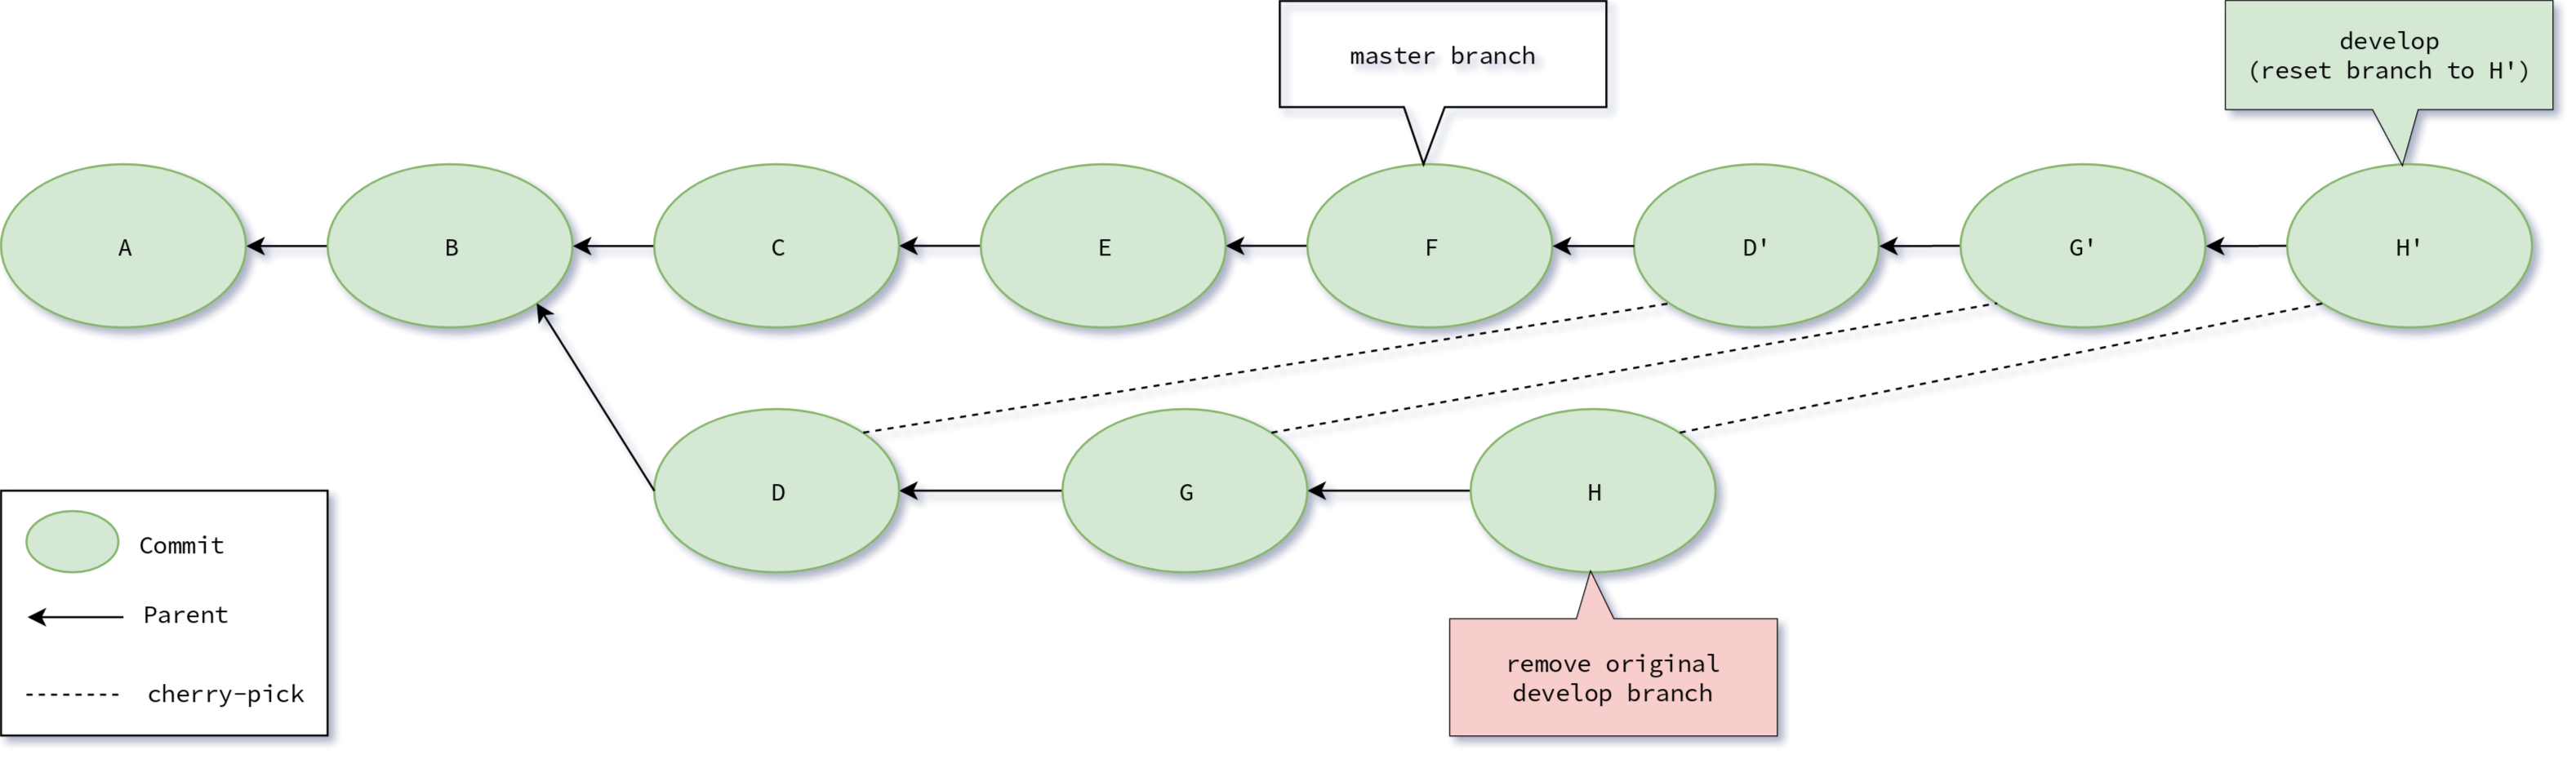
\includegraphics[width=1\textwidth,keepaspectratio]{./images/Rebase-Completed.png}
            }
            \caption{Areas in git}
        \end{center}
    \end{figure}
\end{frame}

